\section{Setup}

We are walking through the
\u{Building a quantum lock using phase kickback}{https://pennylane.ai/qml/demos/tutorial_phase_kickback}
tutorial by Danial Motlagh.

\begin{python}
import pennylane as qml
import numpy as np
import matplotlib.pyplot as plt
qml.drawer.use_style("black_white")
\end{python}

\begin{result}

\end{result}


\section{Conversation}

\subsection{General information}

\begin{ai}
Hi AI. I'd like to study the connection between physics and quantum computing. Please tell me about
the Stern-Gerlach experiment.
\end{ai}

\begin{center}
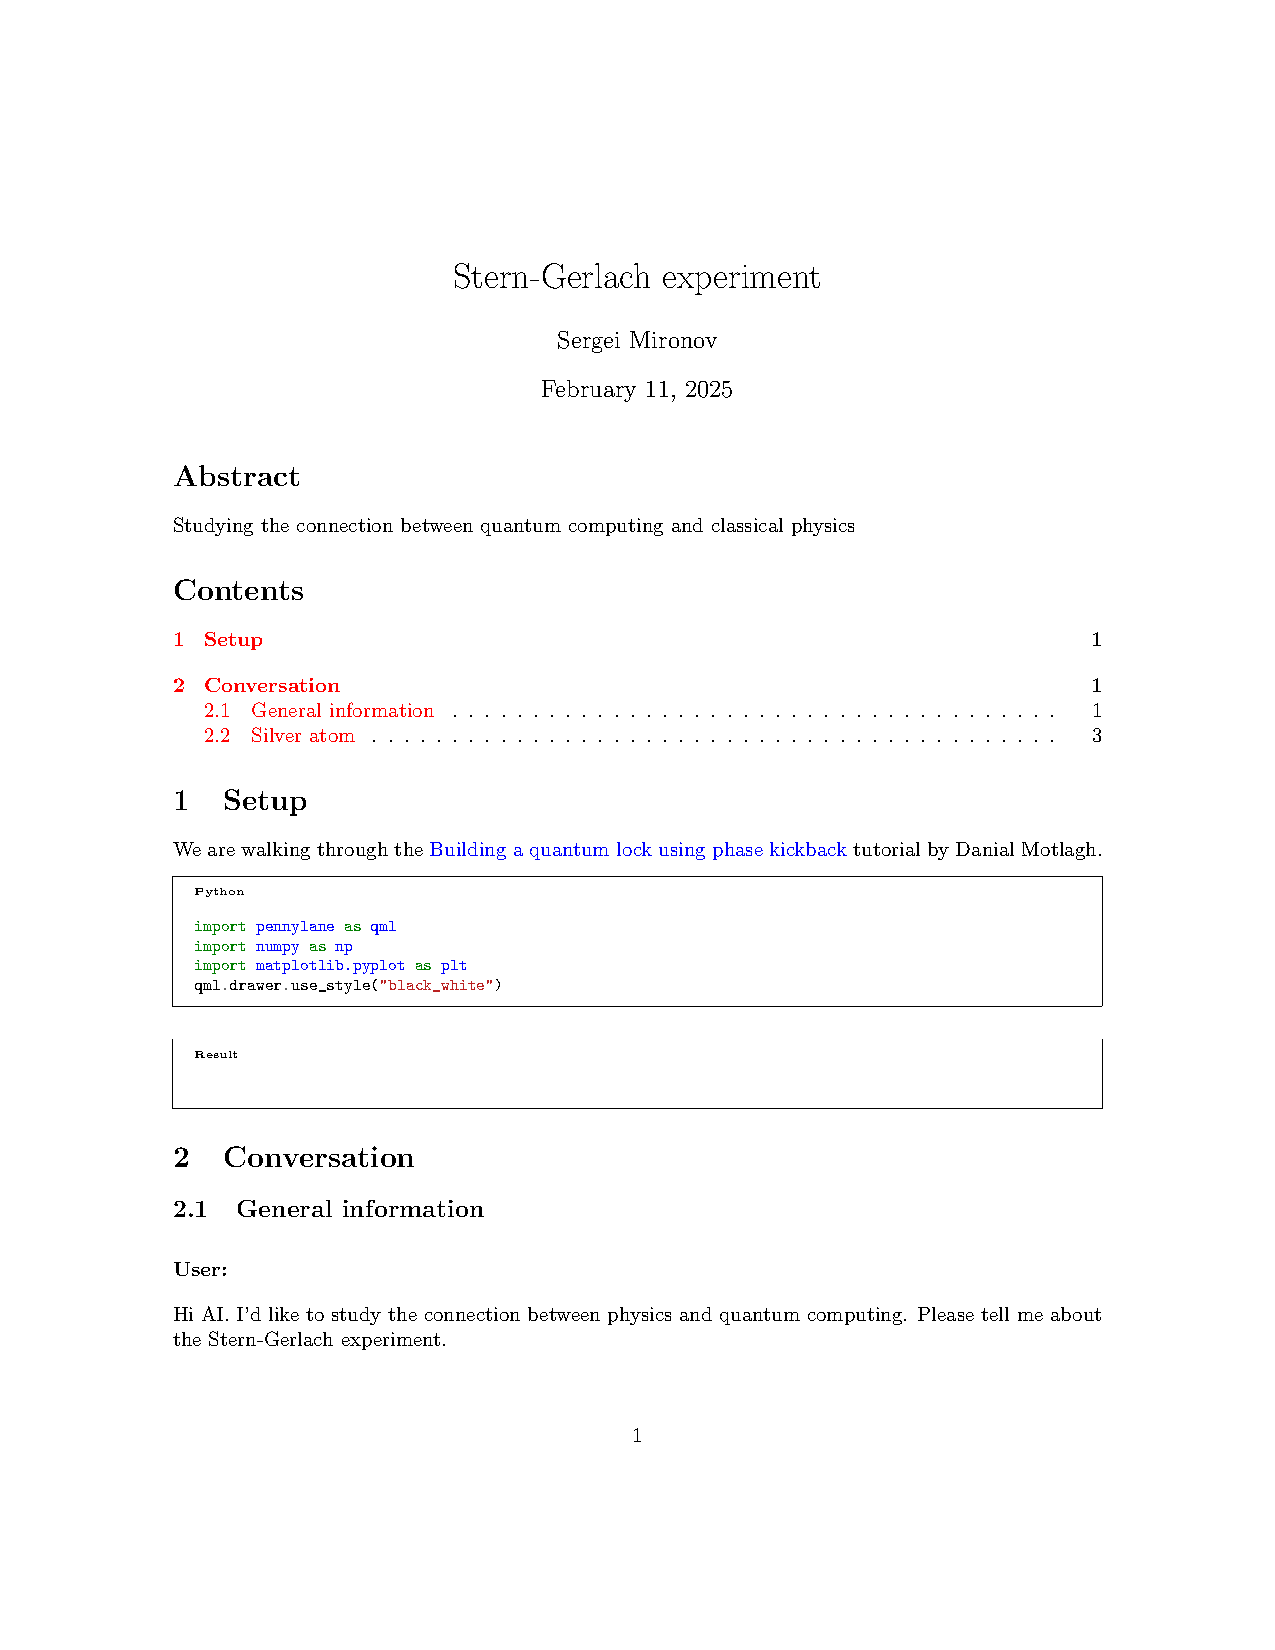
\includegraphics[width=0.8\linewidth]{img/stern-gerlach.png}
\end{center}

\begin{airesult}
The Stern-Gerlach experiment is a fundamental milestone in quantum physics that demonstrates the
quantization of angular momentum, a key concept with profound implications for quantum computing and
quantum mechanics. Here's an overview of the experiment and its significance:

\vsp

\begin{enumerate}
\item \textbf{The Experiment Setup}

The experiment involves sending a beam of silver atoms through a non-uniform magnetic field. These
atoms possess an intrinsic angular momentum called \textit{spin}, which is an internal quantum
property.

\item \textbf{Magnetic Field Interaction}

The inhomogeneous magnetic field interacts with the magnetic moment of the silver atoms, causing
them to be deflected. Classical physics would predict a continuous distribution of deflection
corresponding to a continuous range of angular momenta.

\item \textbf{Quantized Outcomes}

However, the results showed that rather than a continuous spread, the beam splits into discrete
lines, typically two distinct spots. This demonstrated the quantum property of spin, where only
quantized values (in this case, \(\pm \frac{1}{2} \hbar\) for spin-\( \frac{1}{2} \) particles) are
possible.

\item \textbf{Wave-Particle Duality and Quantum Measurement}

The Stern-Gerlach experiment provides direct evidence of the quantized nature of quantum systems and
the principle of quantum superposition. When not measured, the spin state can be a combination of
possible outcomes until a measurement collapses it to a specific value.

\item \textbf{Implications for Quantum Computing}

In quantum computing, the binary nature of spin measurements parallels the operation of qubits,
which exist in superpositions of states until measured. This process underlies quantum gates and
entanglement, essential elements of quantum circuits.

\end{enumerate}

\vsp

The Stern-Gerlach experiment is, therefore, a cornerstone demonstration of quantum mechanics,
highlighting how quantum systems behave fundamentally differently from classical expectations. It
establishes foundational concepts, such as quantum state measurement and spin, that are critical for
understanding and developing quantum technologies like quantum computing.
\end{airesult}


\subsection{Silver atom}


\begin{ai}
Tell me more please about the silver atoms. Why do their spin and magnetic momentum are connected?
\end{ai}

\begin{airesult}
The relationship between spin and magnetic moment in silver atoms, as well as in other atoms, is a
consequence of the underlying quantum mechanics. Here's a deeper look into why these properties are
connected:

\vsp

\begin{enumerate}
\item \textbf{Electron Spin}

Spin is an intrinsic form of angular momentum carried by electrons. It is a purely quantum
mechanical property with no classical analogue. Electrons have a spin of \(\pm \frac{1}{2}\) in
units of \(\hbar\), the reduced Planck constant.

\item \textbf{Magnetic Moment}

The magnetic moment arises from the angular momentum of charged particles. Since electrons have a
charge and also possess spin, they generate a magnetic moment. This is similar to how a classical
charged particle moving in a loop generates a magnetic field.

\item \textbf{Quantum Description of Atomic Magnetic Moment}

In atoms, the total magnetic moment results from both the orbital angular momentum and spin of
electrons. For silver atoms in the Stern-Gerlach experiment, the unpaired outer electron primarily
contributes to the magnetic moment because its motion and spin create a small loop of current with a
north and a south magnetic pole.

\item \textbf{Connection in Silver Atoms}

Silver atoms, specifically, have a single unpaired electron in their outermost shell - the \(5s\)
electron. The majority of its electrons' magnetic moments cancel out because they are paired and
have opposite spins. Therefore, the overall magnetic behavior of the atom is predominantly
determined by this unpaired electron.

\item \textbf{Role in the Stern-Gerlach Experiment}

In the Stern-Gerlach experiment, a beam of neutral silver atoms is used because of this single
unpaired electron, which provides a clear and measurable magnetic moment. When such atoms pass
through a non-uniform magnetic field, the interaction of the unpaired electron’s magnetic moment
with the field causes the beam to split according to the quantized spin states of the electron,
demonstrating the quantization of angular momentum.

\end{enumerate}

\vsp

In quantum mechanics, the intrinsic property of electron spin and its associated magnetic moment are
fundamentally linked, leading to observable phenomena such as the deflection observed in the
Stern-Gerlach experiment. This connection helps illustrate the core quantum principles that also
underpin behaviors in quantum computing, such as the manipulation of qubit states.
\end{airesult}


\begin{ai}
Can you suggest a visualization of a silver atom? I'd like to see its electron configuration. Do you
know a paper which describes this in great details?
\end{ai}

\begin{center}
\includegraphics[width=0.4\linewidth]{img/Ag_bohr_model.png}
\end{center}

\begin{airesult}
To visualize a silver atom and understand its electron configuration, we can create a simple
depiction using the periodic table's information on electron shells and subshells. The electron
configuration gives us insight into which subshells the electrons populate.

The electron configuration of a silver (Ag) atom is:

\vsp

\[
\text{Ag: } [\text{Kr}] \ 4d^{10} \ 5s^1
\]
\vsp

Here's a breakdown of this configuration:

\begin{itemize}
\item The \([ \text{Kr} ]\) indicates that silver's configuration starts like Krypton with 36
electrons.
\item The \(4d^{10}\) subshell is fully filled with 10 electrons.
\item The \(5s^1\) subshell contains one unpaired electron.
\end{itemize}

Given the configuration, the focus for visualizing the atom, especially considering properties
relevant to the Stern-Gerlach experiment or any chemical reactivity, would be on the \(5s^1\)
electron which is the outermost and unpaired electron. This electron contributes the most to the
magnetic moment due to its spin.

To depict this visually, you could draw a nucleus at the center, surrounded by concentric circles
representing shells (energy levels). The inner shells can showcase electrons filling up to Krypton's
configuration. The outermost shell would show the \(5th\) shell with a single electron. This
visualization highlights the presence of the lone unpaired \(5s\) electron.

\vsp

Regarding literature, a recommended resource for detailed descriptions of atomic structures,
including electron configurations, is standard chemistry or quantum mechanics textbooks. For a
detailed scientific paper exploring silver atoms specifically, I suggest looking into articles
published in journals of computational chemistry or atomic physics, such as:

\begin{itemize}
\item "Journal of Chemical Physics"
\item "Physical Review A"
\end{itemize}

These journals often provide in-depth discussions on atomic configurations, potential energy
surfaces, and computational models which can offer detailed insights into the structure and behavior
of specific atoms like silver.
\end{airesult}


\begin{ai}
Can you comment this: In atoms, the total magnetic moment results from both the orbital angular
momentum and spin of electrons. What simplest atom is used in physics textbooks to illustrate this?
\end{ai}

\begin{airesult}
In atoms, the total magnetic moment arises due to contributions from two main sources: the orbital
angular momentum of electrons (which is the result of their motion around the nucleus) and the
intrinsic spin of electrons (a fundamental quantum property). The simplest atom often used in
physics textbooks to illustrate these concepts is the hydrogen atom.

\vsp

\begin{itemize}
\item \textbf{Hydrogen Atom}

  The hydrogen atom is the simplest atom, consisting of a single electron orbiting a single proton.
Despite its simplicity, it is a critical example for studying fundamental quantum mechanical
principles because it exhibits both types of angular momentum: orbital and spin.

\item \textbf{Orbital Angular Momentum}

  The electron in the hydrogen atom moves in quantized orbits around the nucleus, characterized by
the angular momentum quantum number \( l \). The possible values of \( l \) range from 0 to \( n-1
\), where \( n \) is the principal quantum number.

\item \textbf{Spin Angular Momentum}

  The electron also possesses spin, an intrinsic form of angular momentum with only two possible
states: \(+\frac{1}{2}\) (spin-up) and \(-\frac{1}{2}\) (spin-down).

\item \textbf{Magnetic Moment}

  Both the orbital motion and spin contribute to the magnetic moment of the atom, which affects how
it interacts with external magnetic fields. The total magnetic moment is a vector sum of the orbital
and spin magnetic moments.

\item \textbf{Textbook Example}

  The hydrogen atom often serves as the starting point for introducing quantum mechanics concepts.
It provides clear motivation for the development of quantum mechanical models, such as the
Schrödinger equation, and sets the foundation for understanding more complex atomic structures.
\end{itemize}

\vsp

The hydrogen atom's simplicity makes it ideal for exploring these fundamental quantum properties and
their consequences, which can then be extended to understand atoms with more electrons.
\end{airesult}



\begin{ai}
What are angular momentum quantum number \( l \) and  the principal quantum number?
\end{ai}

\begin{airesult}
In quantum mechanics, quantum numbers are used to describe the properties of atomic orbitals and the
electrons within them. Two important quantum numbers are the principal quantum number (\( n \)) and
the angular momentum quantum number (\( l \)). Let's explore both:

\vsp

\begin{itemize}
\item \textbf{Principal Quantum Number (\( n \))}

  \begin{itemize}
  \item Represents the main energy level or shell of an electron in an atom.
  \item Determines the average distance of the electron from the nucleus: higher \( n \) values
    correspond to higher energy levels, and thus electrons are further from the nucleus.
  \item Takes positive integer values: \( n = 1, 2, 3, \ldots \).
  \item The energy of an electron is mainly determined by \( n \), especially in hydrogen-like
    atoms.
  \end{itemize}

\item \textbf{Angular Momentum Quantum Number (\( l \))}

  \begin{itemize}
  \item Associated with the shape of the electron's orbital. It describes the angular distribution
    of the electron cloud.
  \item Takes integer values from 0 to \( n-1 \) for each principal quantum number.
  \item The value of \( l \) determines the subshell or sublevel:
    - \( l = 0 \) corresponds to the \( s \) subshell,
    - \( l = 1 \) corresponds to the \( p \) subshell,
    - \( l = 2 \) corresponds to the \( d \) subshell,
    - \( l = 3 \) corresponds to the \( f \) subshell, and so on.
  \item Each subshell can hold a different number of electrons: \( 2(2l + 1) \).
  \end{itemize}
\end{itemize}

\vsp

The quantum numbers allow us to describe and predict the electron configuration of atoms, which in
turn explains chemical bonding and atomic properties. Both \( n \) and \( l \) are crucial for
understanding the structure of atoms and the placement of electrons within the periodic table.
\end{airesult}


\begin{ai}
In silver, why does the spin of the last electron contribute to the magnetic momentum of the whole
atom? What about its orbital momentum?
\end{ai}

\begin{airesult}
In a silver atom, the contribution of the spin of the last electron to the magnetic moment is
significant because of the specific electron configuration of the atom. Let's explore why the spin
is prominent and the role of orbital momentum:

\vsp

\begin{itemize}
\item \textbf{Electron Configuration of Silver}

  \begin{itemize}
  \item The ground state electron configuration of silver (Ag) is \([ \text{Kr}] \ 4d^{10} \ 5s^1\).
  \item The \(4d^{10}\) subshell is fully filled, and the \(5s\) subshell contains one unpaired
electron.
  \end{itemize}

\item \textbf{Spin Contribution}

  \begin{itemize}
  \item The unpaired \(5s\) electron adds a net spin angular momentum to the atom because it is not
paired with another electron that would negate its magnetic moment.
  \item The spin of an unpaired electron generates a magnetic moment that contributes directly to
the atom's overall magnetic properties.
  \end{itemize}

\item \textbf{Orbital Angular Momentum}

  \begin{itemize}
  \item In the case of the \(5s\) electron, the orbital angular momentum quantum number \(l\) is 0
(since it is in an \(s\) orbital). This means that its contribution to the orbital angular momentum
is zero.
  \item The filled \(4d\) subshell, having all \(d\) orbitals completely filled, effectively cancels
out its orbital angular momentum contributions. Electrons in filled subshells or orbitals align in
such a way that their magnetic moments cancel out.
  \end{itemize}

\item \textbf{Overall Magnetic Moment of Silver}

  \begin{itemize}
  \item Because the \(d\) subshell is fully filled and does not contribute a net magnetic moment,
the only significant contribution comes from the spin of the unpaired \(5s\) electron.
  \item Therefore, the total magnetic moment is primarily due to the spin of this last electron,
rather than from contributions of orbital angular momentum.
  \end{itemize}

\end{itemize}

\vsp

Thus, in an atom like silver, the magnetic properties are dominantly influenced by spin,
particularly when subshells with higher angular momentum are entirely filled, negating orbital
contributions.
\end{airesult}


\begin{ai}
But in Hydrogen we also have a single $s$ electron. What about its orbital momentum?
\end{ai}

\begin{airesult}
In a hydrogen atom, which consists of a single electron orbiting a single proton, both the spin and
orbital angular momenta play important roles in its quantum mechanical description. However, the
specific properties of an \(s\) orbital affect these contributions. Let's delve into this:

\vsp

\begin{itemize}
\item \textbf{Electron in Hydrogen:}

  \begin{itemize}
  \item The electron in hydrogen occupies the \(1s\) orbital in its ground state.
  \item This configuration is denoted as \(1s^1\).
  \end{itemize}

\item \textbf{Orbital Angular Momentum:}

  \begin{itemize}
  \item The orbital angular momentum quantum number \(l\) for an \(s\) orbital is always 0.
  \item Since \(l = 0\), the orbital angular momentum \( L = \sqrt{l(l+1)} \hbar = 0 \).
  \item Consequently, the orbital contribution to the magnetic moment is zero in the ground state of
hydrogen.
  \end{itemize}

\item \textbf{Spin Angular Momentum:}

  \begin{itemize}
  \item The electron has an intrinsic spin characterized by the spin quantum number \( s =
\frac{1}{2} \).
  \item This non-zero spin results in a spin angular momentum \( S = \sqrt{s(s+1)} \hbar \) and
gives rise to a magnetic moment.
  \item The magnetic moment due to spin is not dependent on the orbital type; instead, it arises
from the intrinsic property of the electron itself.
  \end{itemize}

\end{itemize}

\vsp

Overall, in the hydrogen atom, although the \(s\) orbital provides no orbital angular momentum due
to \(l = 0\), the electron’s spin contributes significantly to the atom’s magnetic properties. This
underscores the distinct roles and intrinsic properties of spin and orbital momentum in quantum
mechanics.
\end{airesult}
